\documentclass[11pt, oneside]{article}   	% use "amsart" instead of "article" for AMSLaTeX format
\usepackage{geometry}                		% See geometry.pdf to learn the layout options. There are lots.
\geometry{letterpaper}                   		% ... or a4paper or a5paper or ...
%\geometry{landscape}                		% Activate for rotated page geometry
%\usepackage[parfill]{parskip}    		% Activate to begin paragraphs with an empty line rather than an indent
\usepackage{graphicx}				% Use pdf, png, jpg, or eps§ with pdflatex; use eps in DVI mode
								% TeX will automatically convert eps --> pdf in pdflatex
								\usepackage[bb=boondox]{mathalfa}
\usepackage{mathtools}
\usepackage{amssymb}
\usepackage{amsmath,amsfonts,amsthm} % Math packages
\usepackage{bm}
\usepackage{graphicx}
\usepackage{dsfont}
\graphicspath{ {images/} }

%SetFonts

%SetFonts

\DeclareMathOperator*{\argmin}{arg\,min}
\DeclareMathOperator*{\argmax}{arg\,max}
\newcommand{\horrule}[1]{\rule{\linewidth}{#1}} % Create horizontal rule command with 1 argument of height

\title{
\normalfont \normalsize
\textsc{14D006 Stochastic Models and Optimization} \\ [25pt] % Your university, school and/or department name(s)
\horrule{0.5pt} \\[0.4cm] % Thin top horizontal rule
\huge Problemset 4\\ % The assignment title
\horrule{2pt} \\[0.5cm] % Thick bottom horizontal rule
}

\author{Daniel Bestard, Michael Cameron, Hans-Peter H{\"o}llwirth, Akhil Lohia} % Your name

\date{\normalsize\today} % Today's date or a custom date

\begin{document}
\maketitle


%%%%%%%%
% Problem 1 %
%%%%%%%%
\section{Linear-Quadratic Problem with Forecasts}
First of all let's set up the problem in order to make the proof. The dynamics of the problem is linear function of the form:
$$x_{k+1} = A_{k}x_{k} + B_{k}u_{k} + w_{k}$$
and the cost function is a quadratic function of the form:
$$\underset{w_{k}}{\mathbb{E}}\bigg\{g_{N}(x_{N}) + \sum_{k=0}^{N-1}g_{k}(x_{k},u_{k},w_{k})\bigg\}$$
where
$$g_{N}(x_{N}) = x'_{N}Q_{N}x_{N}$$
$$g_{k}(x_{k},u_{k},w_{k}) = x'_{k}Q_{k}x_{k} + u'_{k}R_{k}u_{k}$$
The matrices $A_{k}$, $B_{k}$, $Q_{k}$ and $R_{k}$ are given and the last two are positive semidefinite symmetric and positive definite symmetric, respectively.\\

The DP-algorithm that solves the minimization problem is:
$$J_{N}(x_{N}) = x'_{N}Q_{N}x_{N}$$
$$J_{k}(x_{k}) = \underset{u_{k}}{min} \underset{w_{k}|y_{k}}{\mathbb{E}} \bigg\{x'_{k}Q_{k}x_{k} + u'_{k}R_{k}u_{k} + J_{k+1}(A_{k}x_{k} + B_{k}u_{k} + w_{k})\bigg\}$$
By induction we get that:
\begin{align*}
J_{N-1}(x_{N-1}) &= \underset{u_{N-1}}{min} \underset{w_{N-1}|y_{N-1}}{\mathbb{E}} \bigg\{x'_{N-1}Q_{N-1}x_{N-1} + u'_{N-1}R_{N-1}u_{N-1} + \\
&+ \big(A_{N-1}x_{N-1} + B_{N-1}u_{N-1} + w_{N-1}\big)'Q_{N}\big(A_{N-1}x_{N-1} + B_{N-1}u_{N-1} + w_{N-1}\big) \bigg\}\\
&= x'_{N-1}Q_{N-1}x_{N-1} + x'_{N-1}A'_{N-1}Q_{N}A_{N-1}x_{N-1} +\\
&+ \underset{u_{N-1}}{min}\bigg\{ u'_{N-1}R_{N-1}u_{N-1} + u'_{N-1}B'_{N-1}Q_{N}B_{N-1}u_{N-1} + 2x'_{N-1}A'_{N-1}Q_{N}B_{N-1}u_{N-1}\bigg\} + \\
&+ \underset{w_{N-1}|y_{N-1}}{\mathbb{E}}\bigg\{ w'_{N-1}Q_{N}w_{N-1} + 2x'_{N-1}A'_{N-1}Q_{N}w_{N-1}\bigg\} + \\
&+ \underset{u_{N-1}}{min} \underset{w_{N-1}|y_{N-1}}{\mathbb{E}} \bigg\{2u'_{N-1}B'_{N-1}Q_{N}w_{N-1}\bigg\}
\end{align*}

By differentiating the previous expression and setting it to 0, we obtain the following result:
$$\big(R_{N-1} + B'_{N-1}Q_{N}B_{N-1}\big)u_{N-1}^{*} = -B'_{N-1}Q_{N}A_{N-1}x_{N-1} - B'_{N-1}Q_{N}\mathbb{E}[w_{N-1}|y_{N-1}]$$

Given the definitions provided previously we can note that the matrix $R_{N-1} + B'_{N-1}Q_{N}B_{N-1}$ is positive definite, which means that we can invert it and obtain the following optimal value:
\begin{align*}
u_{N-1}^{*} &= - \big(R_{N-1} + B'_{N-1}Q_{N}B_{N-1}\big)^{-1}\big(B'_{N-1}Q_{N}A_{N-1}x_{N-1} + B'_{N-1}Q_{N} \mathbb{E}[w_{N-1}|y_{N-1}]\big)\\
&= - \big(R_{N-1} + B'_{N-1}Q_{N}B_{N-1}\big)^{-1}B'_{N-1}Q_{N}\big(A_{N-1}x_{N-1} +\mathbb{E}[w_{N-1}|y_{N-1}]\big)
\end{align*}
Note that the previous expression is already of the form of the expression to be proved. If we substitute back the optimal value $u_{N-1}^{*}$ in $J_{N-1}(x_{N-1})$ and continue doing this we get the general expression provided in the exercise, which is:
$$\mu_{k}^{*}(x_{k},y_{k}) = - \big(R_{k} + B'_{N-1}K_{k+1}B_{k}\big)^{-1}B'_{k}K_{k+1}\big(A_{k}x_{k} + \mathbb{E}[w_{k}|y_{k}]\big) + \alpha_{k}$$
where $K_{k+1}$ is a function of $A_{k}$, $B_{k}$, $Q_{k}$ and $R_{k}$.

%%%%%%%%
% Problem 2 %
%%%%%%%%
\newpage
\section{Computational Assignment on Linear-Quadratic Control}
We consider a horizon of $N=100$ time periods and a discrete time, homogeneous, linear system, i.e.,
$$ x_{k+1} = A x_k + B u_k + w_k$$
with $A = \begin{bmatrix} 1 & 2 \\[0.3em] 3 & 2 \end{bmatrix}$,
       $B = \begin{bmatrix} 4 & 1 \\[0.3em] 2 & 3 \end{bmatrix}$,
and $\{w_k\}$ being a sequence of IID, zero-mean, Gaussian random vectors with diagonal covariance matrix $D$. 
The cost structure is defined as 
\begin{align*}
g_{N}(x_{N}) &= x_N^T C^T C x_N\\
g_{k}(x_{k}) &= x_k^T C^T C x_k + u_k^T R u_k\\
\end{align*}
with $C = \begin{bmatrix} 1 & 3 \end{bmatrix}$ and diagonal, positive-definite input-cost matrix $R$.

\subsection{Controllability and observability conditions}
Note that the matrix $[B, AB] = \begin{bmatrix} 4 & 2 & 7 & 11 \\[0.3em] 1 & 3 & 10 & 10 \end{bmatrix}$ is full rank, thus ensuring controllability. Intuitively, \textit{controllability} means that one is able to move the internal state $x$ of a system from any initial state $x_0$ to any other final state $x_k$ in a finite time period through a control sequence $\{u_k\}$ (ignoring any disturbances). In particular, \textit{controllability} imposes the following structure on the system:
$$
x_k = B u_{k-1} + AB u_{k-2} + ... + A^{k-1}B u_{0} + A^k x_0
$$\\


Furthermore, the observability condition is ensured because matrix $[C^T, A^T C^T] = \begin{bmatrix} 1 & 7 \\[0.3em] 3 & 9 \end{bmatrix}$ is full rank. Intuitively, \textit{observability} means that it is possible to determine the behavior of the entire system through the system's output $\{x_k\}$. In particular, given measurements of the form $z_k = C x_k$, one can infer initial state $x_0$ through the relations
$$
\begin{bmatrix} z_{k-1} \\[0.3em] ... \\[0.3em] z_{1} \\[0.3em] z_{0}  \end{bmatrix} = 
\begin{bmatrix} CA^{k-1} \\[0.3em] ... \\[0.3em] CA \\[0.3em] C  \end{bmatrix} x_0
$$\\


\subsection{Different covariance matrices}
First, we compare the behavior of the system for two covariance matrices for the disturbances, $D_1 = \begin{bmatrix} 1 & 0 \\[0.3em] 0 & 1 \end{bmatrix}$ and $D_2 = \begin{bmatrix} 5 & 0 \\[0.3em] 0 & 6 \end{bmatrix}$, with $D_2$ "much larger" than $D_1$, under optimal control (given by the discrete-time Riccati equation). $R = \begin{bmatrix} 2 & 0 \\[0.3em] 0 & 4 \end{bmatrix}$ and $x_0 = \begin{bmatrix} 1 & 1 \end{bmatrix}^T$ are fixed. \\

\begin{figure}[ht!]
\centering
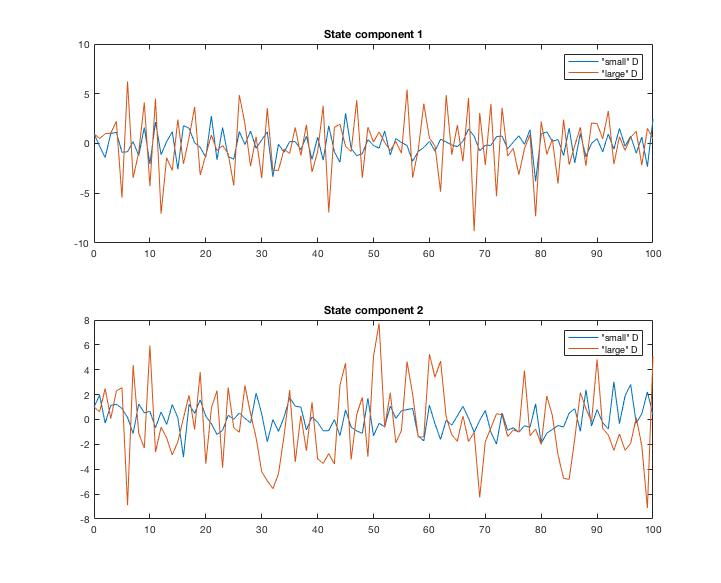
\includegraphics[width=105mm]{../plots/ii.jpg}
\caption{State transitions for covariance matrices $D_1$ (blue) and $D_2$ (orange)}
\end{figure}   

We observe from \textit{Figure 1} that in both cases, the state keeps fluctuating around mean 0. However, as expected the fluctuations are larger for the "larger" covariance matrix $D_2$.

\subsection{Different initial states}
Next, we compare the behavior of the system for two initial conditions, $x_0^{(1)} = \begin{bmatrix} 1 & 1 \end{bmatrix}$ and $x_0^{(2)} = \begin{bmatrix} 5 & 4 \end{bmatrix}$, with $x_0^{(1)}$ "much larger" than $x_0^{(2)}$, under optimal control (given by the discrete-time Riccati equation). $R = \begin{bmatrix} 2 & 0 \\[0.3em] 0 & 4 \end{bmatrix}$ and $D = \begin{bmatrix} 1 & 0 \\[0.3em] 0 & 1 \end{bmatrix}$ are fixed. \\

\begin{figure}[ht!]
\centering
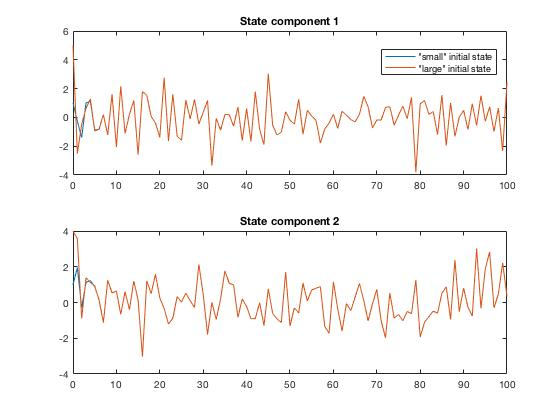
\includegraphics[width=105mm]{../plots/iii.jpg}
\caption{State transitions for initial states $x_0^{(1)}$ (blue) and $x_0^{(2)}$ (orange)}
\end{figure}   

We observe from \textit{Figure 2} that both initial conditions converge to the same state transitions within a few (less than 10) periods.

\subsection{Different input-cost matrices}
Next, we compare the behavior of the system for two input-cost matrices conditions, $R_1 = \begin{bmatrix} 2 & 0 \\[0.3em] 0 & 4 \end{bmatrix}$ and $R_2 = \begin{bmatrix} 18 & 0 \\[0.3em] 0 & 22 \end{bmatrix}$, with $R_2$ "much larger" than $R_1$, under optimal control (given by the discrete-time Riccati equation). $D = \begin{bmatrix} 1 & 0 \\[0.3em] 0 & 1\end{bmatrix}$ and $x_0 = \begin{bmatrix} 1 & 1 \end{bmatrix}^T$ are fixed. \\

\begin{figure}[ht!]
\centering
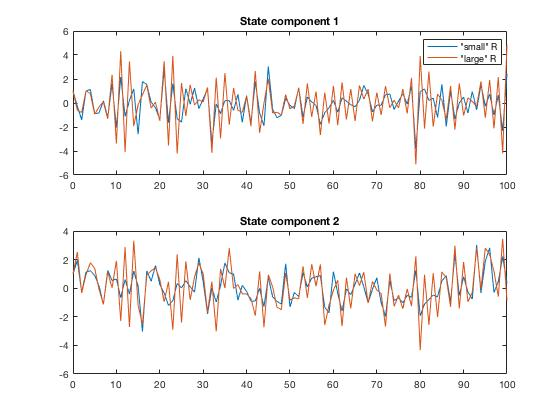
\includegraphics[width=105mm]{../plots/iv.jpg}
\caption{State transitions for input-cost matrices $R_1$ (blue) and $R_2$ (orange)}
\end{figure}   

We observe from \textit{Figure 3} that in both cases, the state keeps fluctuating around mean 0. However, both systems always move into the same direction (up or down), the magnitude of the movement is significantly larger with input-cost matrix $R_2$.

\subsection{Optimal control vs. steady-state control}
Finally, we compare the behavior of the system under optimal control (given by the discrete-time Riccati equation) vs. steady-state control (given by the algebraic Riccati equation). $D = \begin{bmatrix} 1 & 0 \\[0.3em] 0 & 1\end{bmatrix}$, $R = \begin{bmatrix} 2 & 0 \\[0.3em] 0 & 4 \end{bmatrix}$, and $x_0 = \begin{bmatrix} 1 & 1 \end{bmatrix}^T$ are fixed. \\

\begin{figure}[ht!]
\centering
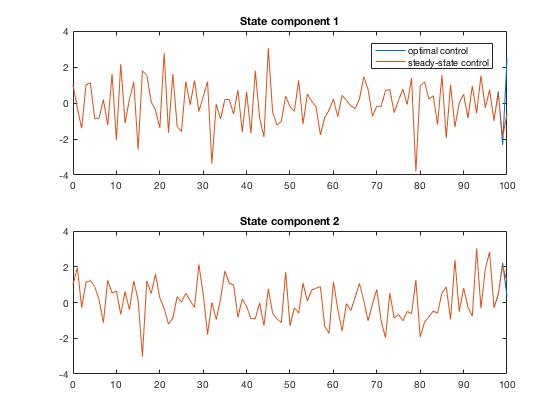
\includegraphics[width=105mm]{../plots/v.jpg}
\caption{State transitions under optimal control (blue) and steady-state control (orange)}
\end{figure}   

We observe from \textit{Figure 4} that under both controls the system has identical state transitions, except for the last few (less than 5) periods. This result shows that the discrete-time Riccati equations converge to the algebraic solution within few iterations.

%%%%%%%%
% Problem 3 %
%%%%%%%%
\section{Asset Selling with Offer Estimation}
This problem is a combination of the standard asset selling problem and the sequential hypothesis testing problem. Our terminal cost in this probelm is the same as in the standard asset selling case. In the final round, we must accept the offer given to us, regardless of the distribution it has come from or if we know which distribution this is. So,  
 \begin{equation}
    x_{N}=
    \begin{cases}
      x_{N}, & \text{if}\ x_{N}\neq T \\
      0, & \text{otherwise}
    \end{cases}
  \end{equation}
 
In the $k^{th}$ period, we have two options, to sell or to wait for the next offer, if we have not already sold the asset. So we must compare our expected return for waiting compared to the returns for selling. As in the standard problem if we sell we will have $(1+r)^{N-k}x_{k}$. However if we wait for the next offer our expected return will be $\mathbb{E}[J_{k+1}(w_{k})| w~distributed~ F_{i}]$. Our expected return for waiting for the next offer depends on our knowledge of the distribution of $w$. Our knowledge of the distribution of $w$ evolves over time with $q_{k}$. \\
As in the sequential hypothesis testing 
 \begin{equation}
    u^{*}_{k}=
    \begin{cases}
      decide~true~ distribution ~is~ F_{1}, & \text{if}\ q_{k} \geq \alpha_{k} \\
      decide ~true~ distribution~ is~ F_{2}, & \text{if}\ q_{k} \leq \beta_{k} \\
      continue, & \text{otherwise}
    \end{cases}
  \end{equation}
where

$$\beta_{k}L_{2}=c+A_{k}(\beta_{k})$$
$$(1-\alpha_{k})L_{1}=c+A_{k}(\alpha_{k})$$
$$A_{k}(q_{k})=\mathbb{E}[J_{k+1}(\frac{q_{k}F_{1}(w_{k+1}}{q_{k}F_{1}(w_{k+1} + (1-q_{k})F_{2}(w_{k+1})})]$$
c is the cost of getting a new observation, which here is how much lower the next offer is compared to the current offer, and L is the loss for incorrrectly guessing the distribution.
Combining the two gives the optimal strategy, when we know the distribution, we sell or wait depending on our expected offers from that distribution. While we dont know the distribution we sell or wait depending on the expected return given the probabilities of us knowing the distribution.
\begin{equation}
    u^{*}_{k}=
    \begin{cases}
      sell, & \text{if}\ q_{k} \geq \alpha_{k} ~\text{and}~ x_{k} \geq \gamma_{k}\\
      wait, & \text{if}\ q_{k} \geq \alpha_{k}~ \text{and} ~x_{k} \leq \gamma_{k}\\
      sell, & \text{if}\ q_{k} \leq \beta_{k} ~\text{and}~ x_{k} \geq \delta_{k}\\
      wait, & \text{if}\ q_{k} \leq \beta_{k}~ \text{and} ~x_{k} \leq \delta_{k}\\
      sell, & \text{if}\ \beta \leq q_{k} \leq ~\alpha_{k}~ \text{and} x_{k} \geq \phi_{k}  \\
      wait, & \text{if}\ \beta \leq q_{k} \leq \alpha_{k}~ \text{and} ~x_{k} \leq \phi_{k}
    \end{cases}
  \end{equation}
where,
$$
\gamma_{k} = \frac{\mathbb{E}[J_{k+1}(w_{k})| w ~distributed~ F_{1}]}{(1+r)^{N-k}} $$
$$
\delta_{k} = \frac{\mathbb{E}[J_{k+1}(w_{k})| w~distributed~  F_{2}]}{(1+r)^{N-k}} $$
$$
\phi_{k} = \frac{\mathbb{E}[J_{k+1}(q_{k}\mathbb{E}_{F_{1}}[w_{k}]+(1-q_{k})\mathbb{E}_{F_{1}}[w_{k}]]}{(1+r)^{N-k}} \\
$$


%%%%%%%%
% Problem 4 %
%%%%%%%%
\section{Inventory Control with Demand Estimation}


%%%%%%%%
% Problem 5 %
%%%%%%%%
\section{Robust Dynamic Programming}
Consider a variation of the basic problem in which we do not have a probabilistic description of uncertainty. Instead, we want to find the closed-loop policy $\pi = \{\mu_0(.),..,\mu_{N-1}(.)\}$ with $\mu_k(x_k) \in U_k(x_k)$ that minimizes the maximum possible cost:
$$
J_{\pi}(x_0) = \max_{w_k \in W_k(x_k,\mu_k(x_k))} \left[ g_N(x_N) + \sum_{k=0}^{N-1} g_k(x_k,\mu_k(x_k), w_k)\right]
$$

\subsection{DP formulation}
Using the principle of optimality, the DP like recursion for this variation of the basic problem looks like:
\begin{align*}
J_{N}(x_{N}) &= g_N(x_N)\\
J_{k}(x_{k}) &= \min_{u_k \in U_k(x_k)} \max_{w_k \in W_k(x_k,\mu_k(x_k))} \left[ g_k(x_k,\mu_k(x_k),w_k) + J_{k+1}(f_k(x_k,\mu_k(x_k),w_k))\right]\\
\end{align*}
Note that, when we compare the DP formulation to the original basic problem, instead of minimizing the expected cost over $w_k$, here we minimize the maximum possible cost that can result from an action $u_k=\mu_k(x_k)$.

\subsection{Reachability of a target tube}
Now assume that at each stage $k$, the state $x_k$ must belong to a given set $X_k$. A cost structure that fits the reachability problem within the general formulation looks as follows:
\begin{align*}
J_{N}(x_{N}) &= 
\begin{cases}
0 & \text{ if } x_N \in X_N\\
1 & \text{ if } x_N \not\in X_N
\end{cases}\\
J_{k}(x_{k}) &= \min_{u_k \in U_k(x_k)} \max_{w_k \in W_k(x_k,\mu_k(x_k))} \left[ J_{k+1}(f_k(x_k,\mu_k(x_k),w_k))\right]\\
\end{align*}

The set $\bar{X}_k$, i.e. the set that we must reach at stage $k$ in order to be able to maintain the state of the system in the desired tube henceforth, can be computed recursively as follows:
\begin{align*}
\bar{X}_N &= X_N\\
\bar{X}_k &= \{x_k: \exists \mu_k(x_k) \in U_k(x_k).\forall w_k\in W_k(x_k,\mu_k(x_k)).f_k(x_k,\mu_k(x_k),w_k) \in \bar{X}_{k+1}\}\\
\end{align*}
For $x_k \in \bar{X}_k$, there must exist at least one action $u_k=\mu_k(x_k)$ in set $U_k(x_k)$ such that every possible outcome $w_k$ in the outcome set $W_k(x_k,\mu_k(x_k))$ takes us to a state $x_{k+1} = f_k(x_k,\mu_k(x_k),w_k) \in \bar{X}_{k+1}$.

\end{document}















